\newpage
\section{SD-card}
The SD-card is responsible for logging data. The data being logged onto the SD-card is both received from the BMS and from the MCU. The data being logged from the BMS is concerning the state of the batteries. The data being logged from the MCU is concerning the power used by the motor.

\subsection{Design}
Through the design phase it was discovered that it is possible to purchase a SD-card module online. This was done and there have no use for designing any hardware for this module.

The only considerations that must be taken into account when communicating with a SD-card, is that it is supplied by 3.3V and the MCU uses. This problem has is taken care of by the SD-card.

As seen on figure \vref{fig:SD} the hardware outlay to communicate with the SD-card is very simple. This is because the add-on board does everything. Furthermore, the specific add-on board here used, is only using the data terminals of the SD-card. There is outputs that are not used with this board, which among other things, sets a pin high when there is a card placed in the holder. 

\begin{figure}[H]
	\centering
	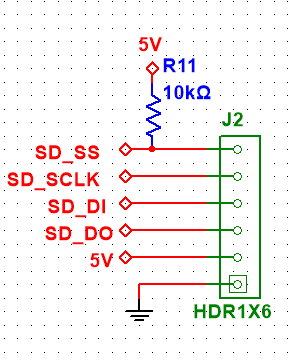
\includegraphics[width=0.4\linewidth]{Hardware/Pictures/SD_card}
	\caption{SD-card schematic}
	\label{fig:SD}
\end{figure}

\newpage
\subsection{Implementation}
The implementation of the SD-card reader is done away from the PCB. This is done so that reader is removable, in case that it is not needed to collect any data in that specific run and thereby not drawing any, albeit small, current.  

The connection between the breakout board(SD-card) used and the controller is via 6 connectors. Supply and ground for the board, and 4 wires used for data transfer. The data transfer works via the SPI protocol, so connections shown on figure \vref{fig:SD} corresponds to the following:

\begin{itemize}
	\item{SD\_SS = Slave select}
	\item{SD\_SCLK = SPI Clock}
	\item{SD\_DI = Master in, Slave out(MISO)}
	\item{SD\_DO = Master Out, Slave in(MOSI)}
\end{itemize}

\subsection{Unity test}
The test is done in correlation with the software test. Since it is a board that is bought, it is assumed to work, which the test showed succesfully. 